\chapter{矩阵方法基础}

\section{矩阵分解}
矩阵分解是线性代数中的一个重要概念,它将一个矩阵分解为多个简单矩阵的乘积。常见的矩阵分解方法包括特征分解、奇异值分解、稀疏分解等。这些分解方法在数值计算、信号处理和机器学习等领域有着广泛的应用。

\subsection{特征分解}
特征分解(Eigenvalue Decomposition)是线性代数中的一个重要概念,对于一个方阵\( \mathbf{A} \in \mathbb{R}^{n \times n} \),其特征值和特征向量满足以下等式:
\begin{equation}
    \mathbf{A} \bm{v} = \lambda \bm{v},
\end{equation}
其中,\( \lambda \) 是特征值,非零向量\( \bm{v} \) 是对应的特征向量。

如果矩阵\( \mathbf{A} \)一共有\( n \)个线性无关的特征向量,这些向量可以构成如下的特征向量矩阵
\[
    \mathbf{V} =
    \begin{bmatrix}
        \bm{v}_1 & \bm{v}_2 & \cdots & \bm{v}_n
    \end{bmatrix},
\]
那么有
\begin{equation}
    \mathbf{A} \mathbf{V} = \mathbf{V} \mathbf{\Lambda},
    \label{eq:eigen-decomposition}
\end{equation}
其中\( \mathbf{\Lambda} \)是一个对角矩阵,其对角线上的元素为对应的特征值,即
\[
    \mathbf{\Lambda} =
    \begin{bmatrix}
        \lambda_1 & 0         & \cdots & 0         \\
        0         & \lambda_2 & \cdots & 0         \\
        \vdots    & \vdots    & \ddots & \vdots    \\
        0         & 0         & \cdots & \lambda_n
    \end{bmatrix}.
\]
对\cref{eq:eigen-decomposition}两边同时右乘\( \mathbf{V}^{-1} \),可以得到
\begin{equation}
    \mathbf{A} = \mathbf{V} \mathbf{\Lambda} \mathbf{V}^{-1}.
    \label{eq:eigen-decomposition-inverse}
\end{equation}
式\cref{eq:eigen-decomposition-inverse}就是矩阵的特征分解形式,而能够被分解的矩阵被称为可对角化矩阵。进一步地,对于对称矩阵,则有\cref{thm:symmetric-eigen-decomposition}所述的特征分解形式。

\begin{theorem}[对称矩阵的特征分解]\label{thm:symmetric-eigen-decomposition}
    如果矩阵\( \mathbf{A} \)是一个对称矩阵,则其特征向量构成的矩阵\( \mathbf{V} \)为正交矩阵,即满足
    \[
        \mathbf{V}^{\mathrm{T}} \mathbf{V} = \mathbf{I}.
    \]
    此时,矩阵有如下特征分解
    \[
        \mathbf{A} = \mathbf{V} \mathbf{\Lambda} \mathbf{V}^{\mathrm{T}}.
    \]
\end{theorem}
\begin{proof}
    设\( \mathbf{A} \)的特征值为\( \lambda_1, \lambda_2, \ldots, \lambda_n \),对应的特征向量为\( \bm{v}_1, \bm{v}_2, \ldots, \bm{v}_n \)。由于\( \mathbf{A} \)是对称矩阵,所以
    \[
        \mathbf{A} \bm{v}_i = \mathbf{A}^{\mathrm{T}} \bm{v}_i = \lambda_i \bm{v}_i.
    \]
    显然,对于任意的\( i \neq j \),都有如下两个等式成立:
    \[
        \begin{split}
            \bm{v}_i^{\mathrm{T}} \mathbf{A} \bm{v}_j & =  \bm{v}_i^{\mathrm{T}} (\mathbf{A} \bm{v}_j)= \lambda_j \bm{v}_i^{\mathrm{T}} \bm{v}_j,                         \\
            \bm{v}_i^{\mathrm{T}} \mathbf{A} \bm{v}_j & = \left(\mathbf{A}^{\mathrm{T}} \bm{v}_i\right)^{\mathrm{T}} \bm{v}_j = \lambda_i \bm{v}_i^{\mathrm{T}} \bm{v}_j.
        \end{split}
    \]
    因此有
    \[
        \lambda_j \bm{v}_i^{\mathrm{T}} \bm{v}_j = \lambda_i \bm{v}_i^{\mathrm{T}} \bm{v}_j.
    \]
    当\( \lambda_i \neq \lambda_j \)时,\( \bm{v}_i^{\mathrm{T}} \bm{v}_j = 0 \),即特征向量正交。当\( \lambda_i = \lambda_j \)时,可以验证,对于任意的线性组合系数\( \alpha, \beta \in \mathbb{R} \),有\(\bm{v} = \alpha \bm{v}_i + \beta \bm{v}_j\)也是特征向量,对应的特征值仍然是\( \lambda_i = \lambda_j \)。

    也就是说,由\( \bm{v}_i \)和\( \bm{v}_j \)张成的平面上的任意向量都是特征向量。从这个平面上可以选出两个正交的特征向量\( \bm{v}_i' \)和\( \bm{v}_j' \),将它们作为新的特征向量。这样,就可以确保所有的特征向量互相之间是正交的。如对所有特征向量都进行归一化,令其模长为一,则特征向量构成的矩阵满足
    \[
        \mathbf{V} \mathbf{V}^{\mathrm{T}} = \mathbf{I}.
    \]
\end{proof}

然而并不是所有的矩阵都可以进行特征分解,对于部分矩阵,其特征向量可能线性相关。此时,矩阵\( \mathbf{V} \)不可逆,因此无法进行特征分解。比如,下方的\( 2 \times 2 \)矩阵:
\[
    \mathbf{A} =
    \begin{bmatrix}
        1 & 1 \\
        0 & 1
    \end{bmatrix}.
\]
设其特征值为\( \lambda \),则有
\[
    \det(\mathbf{A} - \lambda \mathbf{I}) = \det\left(
    \begin{bmatrix}
            1 - \lambda & 1           \\
            0           & 1 - \lambda
        \end{bmatrix}\right) = (1 - \lambda)^2 = 0.
\]
因此,该矩阵的两个特征值都是1,对应的特征向量相同,都为
\[
    \bm{v} =
    \begin{bmatrix}
        1 \\
        0
    \end{bmatrix}.
\]
对于这样不可对角化的矩阵,我们可以进行广义特征分解,将矩阵分解为若尔当标准型(Jordan form):
\begin{theorem}[广义特征分解] \label{thm:jordan-decomposition}
    对于任意的\( n \times n \)矩阵\( \mathbf{A} \),存在一个可逆矩阵\( \mathbf{P} \)和一个分块对角矩阵\( \mathbf{J} \),使得
    \[
        \mathbf{A} = \mathbf{P} \mathbf{J} \mathbf{P}^{-1}.
    \]
    分块对角矩阵\( \mathbf{J} \)有如下形式
    \[
        \mathbf{J} =
        \begin{bmatrix}
            J_1    & 0      & \cdots & 0      \\
            0      & J_2    & \cdots & 0      \\
            \vdots & \vdots & \ddots & \vdots \\
            0      & 0      & \cdots & J_k
        \end{bmatrix},
    \]
    其中每个\( J_i \)是一个若尔当块(Jordan block),其形式为
    \[
        J_i =
        \begin{bmatrix}
            \lambda_i & 1         & 0         & \cdots & 0         \\
            0         & \lambda_i & 1         & \cdots & 0         \\
            0         & 0         & \lambda_i & \ddots & 0         \\
            \vdots    & \vdots    & \vdots    & \ddots & 1         \\
            0         & 0         & 0         & \cdots & \lambda_i
        \end{bmatrix}.
    \]
\end{theorem}
考虑到本书后续的内容不涉及广义特征分解,这里不再给出\cref{thm:jordan-decomposition}的证明。除了广义特征分解外,我们还可以使用其他的矩阵分解方法来处理不可对角化的矩阵,比如下一小节给出的奇异值分解。

\begin{example}
    设有三座城市,且这三座城市之间人口流动的情况可以用一个矩阵来表示:
    \[
        \mathbf{P} =
        \begin{bmatrix}
            0.5 & 0.2 & 0.1 \\
            0.3 & 0.5 & 0.4 \\
            0.2 & 0.3 & 0.5
        \end{bmatrix},
    \]
    其中,\( P_{ij} \)表示单位时间内,从城市\( j \)流入到城市\( i \)的人口比例。比如\( P_{11} = 0.5 \),表明经过一个单位时间,有50\%的人口仍然留在城市1,\( P_{12} = 0.2 \)表示第2个城市20\%的人口会流动到城市1。请求解以下问题:
    \begin{enumerate}
        \item 假设初始时刻,三个城市的人口都为1000人,请计算经过一个单位时间后,各个城市的人口分布情况。
        \item 请计算经过足够长的时间后,各个城市的人口分布情况。
    \end{enumerate}
\end{example}
\begin{solution}
    \begin{enumerate}
        \item 记初始时刻三个城市的人口数量为如下向量
              \[
                  \bm{x}_0 =
                  \begin{bmatrix}
                      1000 \\
                      1000 \\
                      1000
                  \end{bmatrix}.
              \]
              则经过一个单位时间后,各个城市的人口数量为
              \[
                  \bm{x}_1 = \mathbf{P} \bm{x}_0 =
                  \begin{bmatrix}
                      0.5 & 0.2 & 0.1 \\
                      0.3 & 0.5 & 0.4 \\
                      0.2 & 0.3 & 0.5
                  \end{bmatrix}
                  \begin{bmatrix}
                      1000 \\
                      1000 \\
                      1000
                  \end{bmatrix} =
                  \begin{bmatrix}
                      800  \\
                      1200 \\
                      1000
                  \end{bmatrix}.
              \]

        \item 设\( \bm{x}_n \)为经过\( n \)个单位时间后,各个城市的人口分布情况。则有
              \[
                  \bm{x}_n = \mathbf{P} \bm{x}_{n-1} = \mathbf{P}^n \bm{x}_0.
              \]
              又因为\( \mathbf{P} \)有如下特征分解
              \[
                  \mathbf{P} = \mathbf{V} \mathbf{\Lambda} \mathbf{V}^{-1},
              \]
              其中
              \[
                  \mathbf{V} \approx
                  \begin{bmatrix}
                      0.3995 & -0.8090 & 0.3090  \\
                      0.7068 & 0.3090  & -0.8090 \\
                      0.5839 & 0.5000  & 0.5000
                  \end{bmatrix}, \quad \mathbf{\Lambda} \approx
                  \begin{bmatrix}
                      1 & 0      & 0      \\
                      0 & 0.3618 & 0      \\
                      0 & 0      & 0.1382
                  \end{bmatrix}.
              \]
              因此,当\( n \)趋向于无穷大时,\( \mathbf{P}^n \)的收敛于一个矩阵,其近似值为
              \[
                  \lim_{n \to \infty} \mathbf{P}^n = \lim_{n \to \infty} \mathbf{V} \mathbf{\Lambda}^n \mathbf{V}^{-1} = \mathbf{V}
                  \begin{bmatrix}
                      1 & 0 & 0 \\
                      0 & 0 & 0 \\
                      0 & 0 & 0
                  \end{bmatrix} \mathbf{V}^{-1} \approx
                  \begin{bmatrix}
                      0.2364 & 0.2364 & 0.2364 \\
                      0.4182 & 0.4182 & 0.4182 \\
                      0.3455 & 0.3455 & 0.3455
                  \end{bmatrix}.
              \]
              于是,经过足够长的时间后,各个城市的人口分布情况为
              \[
                  \bm{x}_\infty = \lim_{n \to \infty} \bm{x}_n = \lim_{n \to \infty} \mathbf{P}^n \bm{x}_0 \approx
                  \begin{bmatrix}
                      709.1  \\
                      1254.5 \\
                      1036.4
                  \end{bmatrix}.
              \]

    \end{enumerate}
\end{solution}

\subsection{奇异值分解}

奇异值分解(Singular Value Decomposition, SVD)是线性代数中一个非常重要的矩阵分解工具,被广泛应用于信号处理、统计学、机器学习、图像压缩等领域。相比于特征分解,奇异值分解不要求矩阵是可逆的,可以应用于任意形状的矩阵,具体见下方的定理。

\begin{theorem}
    对于任意的矩阵\( \mathbf{A} \in \mathbb{R}^{m \times n} \),都存在一个奇异值分解:
    \[
        \mathbf{A} = \mathbf{U} \mathbf{S} \mathbf{V}^{\mathrm{T}},
    \]
    其中,\( \mathbf{U} \in \mathbb{R}^{m \times m} \)是一个正交矩阵,其列向量被称作左奇异向量;\( \mathbf{V} \in \mathbb{R}^{n \times n} \)是一个正交矩阵,其列向量被称作右奇异向量;\( \mathbf{S} \in \mathbb{R}^{m \times n} \)是一个对角矩阵,其对角线上的元素被称作奇异值(Singular Values)。
\end{theorem}
\begin{proof}
    不妨假设\( m \geq n \),则\( \mathbf{A}^{\mathrm{T}} \mathbf{A} \) 为一个\( n \times n \)的对称矩阵。根据\cref{thm:symmetric-eigen-decomposition},存在一个正交矩阵\( \mathbf{V} \)和一个对角矩阵\( \mathbf{\Lambda} \),使得
    \[
        \mathbf{A}^{\mathrm{T}} \mathbf{A} = \mathbf{V} \mathbf{\Lambda} \mathbf{V}^{\mathrm{T}}.
    \]
    可以验证,\( \mathbf{\Lambda} \)的对角元素必然是非负的。因此不妨将矩阵\( \mathbf{A}^{\mathrm{T}} \mathbf{A} \)的特征值记作\( \lambda_i^2 \)。令\( \bm{v}_i \)为\( \mathbf{V} \)的第\( i \)列向量,并令
    \[
        \bm{u}_i = \frac{\mathbf{A} \bm{v}_i}{\|\mathbf{A} \bm{v}_i\|} = \frac{\mathbf{A} \bm{v}_i}{\sqrt{\bm{v}_i^{\mathrm{T}} \mathbf{A}^{\mathrm{T}} \mathbf{A} \bm{v}_i}} = \frac{1}{\lambda_i} \mathbf{A} \bm{v}_i.
    \]
    则有
    \begin{equation}\label{eq:svd_proof1}
        \bm{u}_i^{\mathrm{T}} \mathbf{A} \bm{v}_i = \frac{1}{\lambda_i} \bm{v}_i^{\mathrm{T}} \mathbf{A}^{\mathrm{T}} \mathbf{A} \bm{v}_i = \frac{1}{\lambda_i} \lambda_i^2 = \lambda_i.
    \end{equation}
    并且,可以验证对于任意的\( i \neq j  \)且\( i, j \leq n \),都有
    \begin{equation}\label{eq:svd_proof2}
        \bm{u}_i^{\mathrm{T}} \mathbf{A} \bm{v}_j = \frac{1}{\lambda_i} \bm{v}_i^{\mathrm{T}} \mathbf{A}^{\mathrm{T}} \mathbf{A} \bm{v}_j = 0.
    \end{equation}
    注意到,\( \bm{u}_j = \frac{1}{\lambda_j} \mathbf{A} \bm{v}_j \),因此还可以得出\( \bm{u}_i \)和\( \bm{u}_j \)是正交的。

    不妨构造如下的矩阵
    \[
        \mathbf{U} =
        \begin{bmatrix}
            \bm{u}_1 & \bm{u}_2 & \cdots & \bm{u}_n & \bm{u}_{n+1} & \cdots & \bm{u}_m
        \end{bmatrix} \in \mathbb{R}^{m \times m},
    \]
    对于其中的列向量,当\( 1 \leq i \leq n \)时,有\( \bm{u}_i = \frac{\mathbf{A} \bm{v}_i}{\|\mathbf{A} \bm{v}_i\|} \);而当\( n + 1 \leq i \leq m \)时,可以令\( \bm{u}_i \)为\( \mathbf{A} \)的零空间中的任意向量,只需满足构成的矩阵\( \mathbf{U} \)是一个正交矩阵即可。此时,可以验证,对于任意的\( i \neq j  \)且\( i \leq n, j > n\),都有
    \begin{equation}\label{eq:svd_proof3}
        \bm{u}_i^{\mathrm{T}} \mathbf{A} \bm{v}_j = 0.
    \end{equation}

    综上所述,结合\cref{eq:svd_proof1,eq:svd_proof2,eq:svd_proof3},可以得到
    \[
        \bm{u}_i^{\mathrm{T}} \mathbf{A} \bm{v}_j =
        \begin{cases}
            \lambda_i, & i = j,    \\
            0,         & i \neq j.
        \end{cases}
    \]
    因此,对于构造的矩阵\( \mathbf{U} \),可以验证其满足
    \[
        \mathbf{U}^{\mathrm{T}} \mathbf{A} \mathbf{V} =
        \begin{bmatrix}
            \sqrt{\mathbf{\Lambda}} \\
            \mathbf{0}
        \end{bmatrix} \in \mathbb{R}^{m \times n},
    \]
    其中\( \sqrt{\mathbf{\Lambda}} \)是\( \mathbf{\Lambda} \)的开平方,也是一个对角矩阵,其对角线上的元素为\( \lambda_i \),而\( \mathbf{0} \)是一个\( (m - n) \times n \)的全零矩阵。记该分块矩阵为\( \mathbf{S} \), 并对上式两边同时左乘\( \mathbf{U} \),右乘\( \mathbf{V}^{\mathrm{T}} \),即可得到
    \[
        \mathbf{A} = \mathbf{U} \mathbf{S} \mathbf{V}^{\mathrm{T}}.
    \]
\end{proof}

有意思的是,对于对称矩阵,其奇异值分解和特征分解是等价的。不妨设有对称矩阵\( \mathbf{A} \in \mathbb{R}^{n \times n} \),其SVD分解为
\[
    \mathbf{A} = \mathbf{U} \mathbf{S} \mathbf{V}^{\mathrm{T}}.
\]
又因为\( \mathbf{A}^{\mathrm{T}} = \mathbf{A} \),因此有
\[
    \mathbf{A} = \mathbf{A}^{\mathrm{T}}= \left( \mathbf{U} \mathbf{S} \mathbf{V}^{\mathrm{T}} \right)^{\mathrm{T}} = \mathbf{V} \mathbf{S}^{\mathrm{T}} \mathbf{U}^{\mathrm{T}}.
\]
注意到\( \mathbf{S} \) 是一个\( n \times n \)的对角矩阵,所以\( \mathbf{S}^{\mathrm{T}}  = \mathbf{S} \),至此可以得到如下等式
\[
    \mathbf{A} = \mathbf{U} \mathbf{S} \mathbf{V}^{\mathrm{T}} = \mathbf{V} \mathbf{S} \mathbf{U}^{\mathrm{T}}.
\]
观察上式,不难发现\( \mathbf{U} =  \mathbf{V} \)。此时,对称矩阵\( \mathbf{A} \)的特征分解可以写为\( \mathbf{A} = \mathbf{V} \mathbf{S} \mathbf{V}^{\mathrm{T}} \),因此对称矩阵的奇异值分解和特征分解是等价的。

除此以外,SVD分解实际上提供了一种对矩阵进行低秩近似的方法。考虑如下优化问题:
\begin{equation}
    \begin{cases}
        \min_{\mathbf{B}} & \|\mathbf{A} - \mathbf{B}\|_{\mathrm{F}}^2 \\
        \text{s.t.}       & \text{rank}(\mathbf{B}) = k
    \end{cases}.
    \label{eq:sparse-approximation}
\end{equation}
其中\( \|\cdot\|_F \)表示矩阵的Frobenius范数。通过计算\( \mathbf{A} \)的SVD分解,并保留最大的\( k \)个奇异值和对应的奇异向量,即截断 SVD (Truncated SVD)分解,可以得到该优化问题的最优解:
\begin{equation}
    \mathbf{B} = \sum_{i=1}^{k} \lambda_i \bm{u}_i \bm{v}_i^{\mathrm{T}},
    \label{eq:sparse-approximation-solution}
\end{equation}
其中\( \lambda_i \)是矩阵\( \mathbf{A} \)第\( i \)大的奇异值,\( \bm{u}_i \)和\( \bm{v}_i \)分别是对应的左奇异向量和右奇异向量。具体证明不再展开,请读者自行推导。

\begin{example}
    对于如\cref{fig_cat_gray}所示的灰度图像,可以将其看作是一个\( 200 \times 300 \)的矩阵,请利用奇异值分解对其进行压缩处理。
    \begin{figure}[htb!]
        \centering
        
\includegraphics[width=.3\textwidth]{./img/matrix/cat_g.jpg}
        \caption{原始灰度图像}
        \label{fig_cat_gray}
    \end{figure}
\end{example}
\begin{solution}
    直接对图像矩阵进行奇异值分解,得到
    \[
        \mathbf{A} = \mathbf{U} \mathbf{S} \mathbf{V}^{\mathrm{T}}.
    \]
    其中\( \mathbf{S} \)的对角线元素从大到小排列绘制的曲线如\cref{fig_singular_values}所示。从图中可以看到,奇异值数值迅速下降,这表明大部分信息都集中在较大的奇异值对应的特征向量上。
    \begin{figure}[htb!]
        \centering
        \includegraphics[width=.6\textwidth]{./img/matrix/cat_svd.tikz}
        \caption{奇异值的大小}
        \label{fig_singular_values}
    \end{figure}

    因此,我们可以通过保留前\( k \)个奇异值来实现图像的压缩。具体而言,设\( k \)为保留的奇异值个数,则压缩后的图像矩阵为原始矩阵的低秩近似:
    \[
        \mathbf{A}_{\text{compressed}} = \mathbf{U}_{k} \mathbf{S}_{k} \mathbf{V}_{k}^{\mathrm{T}},
    \]
    其中\( \mathbf{U}_k \in \mathbb{R}^{m \times k} \)是\( \mathbf{U} \)的前\( k \)列,\( \mathbf{S}_k \in \mathbb{R}^{k \times k} \)是\( \mathbf{S} \)的前\( k \)行和前\( k \)列,\( \mathbf{V}_k \in \mathbb{R}^{n \times k} \)是\( \mathbf{V} \)的前\( k \)列。

    通过调整\( k \)的值,可以控制压缩后的图像质量和文件大小,如\cref{fig_compressed_images}所示。可以看到,随着\( k \)的增大,图像质量逐渐提高,当\( k=50 \)时,图像质量已经非常接近原始图像,此时,对应的三个矩阵的元素个数(\( 200 \times 50 + 50 + 300 \times 50 \))大约只有原始矩阵元素个数(\( 200 \times 300 \))的41\%。
    \begin{figure}[htb!]
        \centering
        \begin{subfigure}{.3\textwidth}
            \centering
            
\includegraphics[width=.9\textwidth]{./img/matrix/cat_approx1.jpg}
            \caption{}
            \label{fig_compressed_images_1}
        \end{subfigure}
        \begin{subfigure}{.3\textwidth}
            \centering
            
\includegraphics[width=.9\textwidth]{./img/matrix/cat_approx2.jpg}
            \caption{}
            \label{fig_compressed_images_2}
        \end{subfigure}
        \begin{subfigure}{.3\textwidth}
            \centering
            
\includegraphics[width=.9\textwidth]{./img/matrix/cat_approx3.jpg}
            \caption{}
            \label{fig_compressed_images_3}
        \end{subfigure}
        \caption{奇异值分解压缩后的图像 (a) \( k = 10 \) (b) \( k = 20 \) (c) \( k = 50 \)}
        \label{fig_compressed_images}
    \end{figure}
\end{solution}

\subsection{稀疏分解}
稀疏分解(Sparse Decomposition)是指将一个观测向量表示为一个字典矩阵与一个稀疏系数向量的乘积。具体而言,字典矩阵(Dictionary Matrix)由一组基向量组成,其中每一列(或每一行,取决于具体定义与应用场景)均可视为一个基向量。该矩阵可理解为由若干基础特征模板构成的集合。通过与稀疏系数向量相乘,仅需选择少量的基向量即可近似重构原始数据,从而实现对信号或数据的高效表示与压缩。这种表示方式不仅能够显著降低存储开销,还可有效提升运算效率,在信号处理、模式识别、图像重建等领域具有广泛的应用价值。

稀疏分解对应的优化问题可以表示为
\begin{equation}
    \begin{cases}
        \min_{\bm{x}} & \left\| \bm{x} \right\|_0  \\
        \text{s.t.}   & \mathbf{D} \bm{x} = \bm{y}
    \end{cases},
    \label{eq:sparse-decomposition}
\end{equation}
其中,\( \bm{y} \in \mathbb{R}^m \)是观测向量,\( \mathbf{D} \in \mathbb{R}^{m \times n} \)是字典矩阵。一般来说,\( n \gg m \),这意味着方程\( \mathbf{D} \bm{x} = \bm{y} \)可能有多个甚至无穷多个解。而稀疏分解则是希望找到其中最稀疏的那个解,即使得系数向量\( \bm{x} \)的非零元素个数最少。当存在噪声时,等式\( \mathbf{D} \bm{x} = \bm{y} \)可能无法完全满足,此时可以将约束条件改为
\begin{equation}
    \begin{cases}
        \min_{\bm{x}} & \left\| \bm{x} \right\|_0                                     \\
        \text{s.t.}   & \left\| \bm{y} - \mathbf{D} \bm{x} \right\|_2 \leq \epsilon^2
    \end{cases}.
    \label{eq:sparse-decomposition-noisy}
\end{equation}

然而,优化问题 \cref{eq:sparse-decomposition} 中的 \( \ell_0 \)-范数是非凸且不连续的,使得该问题属于 NP-hard 问题,难以直接求解。因此,通常采用以下近似方法进行求解:

\begin{enumerate}[label=\arabic*.]
    \item \textbf{基追踪(Basis Pursuit, BP)}:将 \( \ell_0 \)-范数替换为其凸包 \( \ell_1 \)-范数,转化为如下凸优化问题:
          \begin{equation}
              \begin{cases}
                  \min_{\bm{x}} \quad & \left\| \bm{x} \right\|_1                                                                         \\
                  \text{s.t.} \quad   & \mathbf{D} \bm{x} = \bm{y} \text{ 或 } \left\| \bm{y} - \mathbf{D} \bm{x} \right\|_2 \leq \epsilon
              \end{cases}.
              \label{eq:basis-pursuit}
          \end{equation}
          在满足一定条件,如限制性等距条件(Restricted Isometry Property)时,该方法能够准确恢复原始的稀疏解。并且,可以通过成熟的线性规划(Linear Programming)或二阶锥规划(Second-Order Cone Programming)等算法高效求解。

    \item \textbf{LASSO(Least Absolute Shrinkage and Selection Operator)}:通过引入 \( \ell_1 \)-范数正则项,构造如下优化模型:
          \begin{equation}
              \min_{\bm{x} \in \mathbb{R}^n} \left\| \bm{y} - \mathbf{D} \bm{x} \right\|_2^2 + \lambda \left\| \bm{x} \right\|_1,
              \label{eq:lasso}
          \end{equation}
          其中,\( \lambda > 0 \) 是正则化参数,用于权衡数据拟合精度与解的稀疏性。LASSO 更适用于存在观测噪声的实际应用场景,可以通过坐标下降法(Coordinate Descent)、交替方向乘子法(Alternating Direction Method of Multipliers, ADMM)等算法高效求解。
\end{enumerate}

除了上述方法,稀疏分解还可以采用匹配追踪(Matching Pursuit)、正交匹配追踪(Orthogonal Matching Pursuit, OMP)、迭代阈值法(Iterative Thresholding)等方法进行求解。这些方法在计算效率与重构精度之间提供了多样化的折中方案,可根据具体应用需求灵活选取。

将稀疏分解拓展到矩阵的情形,可以得到\( k \)-SVD(\( k \)-Sparse Singular Value Decomposition)模型。该模型假设矩阵的奇异值分解可以表示为一个稀疏系数向量与字典矩阵的乘积。具体而言,给定一个矩阵 \( \mathbf{Y} \in \mathbb{R}^{m \times n} \),对应的 \( k \)-SVD 优化问题可以表示为
\begin{equation}
    \begin{cases}
        \min_{\mathbf{D}, \mathbf{X}} & \left\| \mathbf{Y} - \mathbf{D} \mathbf{X} \right\|_{\mathrm{F}}^2 \\
        \text{s.t.}                   & \left\| \bm{x}_i \right\|_0 = 1, \quad \forall i = 1, \ldots, n
    \end{cases},
    \label{eq:k-svd}
\end{equation}
其中,\( \mathbf{D} \in \mathbb{R}^{m \times k} \)是字典矩阵,\( \mathbf{X} =
\begin{bsmallmatrix} \bm{x}_1 & \bm{x}_2 & \cdots & \bm{x}_n
\end{bsmallmatrix} \in \mathbb{R}^{k \times n} \)是稀疏系数矩阵。\( k \)-SVD是对聚类算法\( k \)-均值(\( k \)-Means)的一种推广,其中字典矩阵的列向量对应聚类中心,而稀疏系数矩阵\( \mathbf{X} \)则包含了聚类结果。

除此以外,稀疏分解的矩阵推广还有另一种形式,即鲁棒主成分分析(Robust Principal Component Analysis, RPCA)。RPCA假设观测矩阵可以分解为一个低秩矩阵和一个稀疏矩阵的和。具体而言,给定一个矩阵 \( \mathbf{Y} \in \mathbb{R}^{m \times n} \),RPCA 的优化问题可以表示为
\begin{equation}
    \begin{cases}
        \min_{\mathbf{L}, \mathbf{S}} & \left\| \mathbf{L} \right\|_* + \lambda \left\| \operatorname{vec}(\mathbf{S})\right\|_1 \\
        \text{s.t.}                   & \mathbf{Y} = \mathbf{L} + \mathbf{S}
    \end{cases},
    \label{eq:rpca}
\end{equation}
其中,\( \mathbf{L} \in \mathbb{R}^{m \times n} \)是低秩矩阵,\( \left\| \cdot \right\|_* \)表示核范数,\( \mathbf{S} \in \mathbb{R}^{m \times n} \)是稀疏矩阵,\( \left\| \operatorname{vec}(\cdot)\right\|_1 \)表示将矩阵展开为向量后的 \( \ell_1 \)-范数,即矩阵所有元素的绝对值之和。由于稀疏项的存在,RPCA能够有效提取数据中的异常,同时保留主要的低秩结构。

\begin{example}
    请对如\cref{fig_rpca_example}所示的包含椒盐噪声的图像矩阵进行去噪处理。
    \begin{figure}[htb!]
        \centering
        
\includegraphics[width=.3\textwidth]{./img/matrix/cat_noisy.jpg}
        \caption{包含椒盐噪声的图像}
        \label{fig_rpca_example}
    \end{figure}
\end{example}
\begin{solution}
    不难发现,椒盐噪声对应的矩阵是一个稀疏矩阵,而原始图像矩阵则是一个低秩矩阵。因此,我们可以使用鲁棒主成分分析(RPCA)来对其进行去噪处理。算法结果如\cref{fig_rpca_result}所示,可以看到,所分离出的低秩矩阵基本对应无噪声的图像,而稀疏矩阵则对应椒盐噪声部分。
    \begin{figure}[htb!]
        \centering
        \begin{subfigure}{.3\textwidth}
            \centering
            
\includegraphics[width=.9\textwidth]{./img/matrix/cat_low_rank.jpg}
            \caption{}
            \label{fig_rpca_result_1}
        \end{subfigure}
        \begin{subfigure}{.3\textwidth}
            \centering
            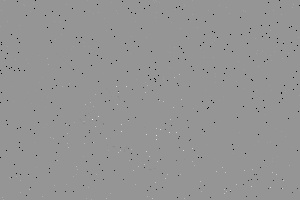
\includegraphics[width=.9\textwidth]{./img/matrix/cat_sparse.jpg}
            \caption{}
            \label{fig_rpca_result_2}
        \end{subfigure}
        \caption{鲁棒主成分分析结果 (a) 低秩矩阵 (b) 稀疏矩阵}
        \label{fig_rpca_result}
    \end{figure}
\end{solution}

\maybeNewPage

\section{矩阵微分}

\subsection{实矩阵微分}
普通的求导想必大家都很熟悉,比如对于标量函数$f(x)$, 其关于$x$的导数可以表示为\( \frac{\partial f(x)}{\partial x} \)。 而函数不仅仅可以是关于标量的函数,也可以是关于向量甚至矩阵的函数。比如,一个二元函数\( f(x_1, x_2) \)则可以看作是关于向量\( \bm{x} = \begin{bsmallmatrix} x_1 & x_2 \end{bsmallmatrix}^{\mathrm{T}} \)的一个函数\( f(\bm{x}) \)。自然地,我们也可以求解其关于向量\( \bm{x} \)的导数。具体而言,我们有如下定义。

\begin{definition}[标量关于向量求导]
    对于向量$\bm{x} \in \mathbb{R}^{n \times 1}$,有映射\( f: \mathbb{R}^{n \times 1} \rightarrow \mathbb{R} \),则定义其关于向量\( \bm{x} \)的导数为
    \[
        \frac{\partial f(\bm{x})}{\partial \bm{x}}  =
        \begin{bmatrix}
            \frac{\partial f(\bm{x})}{\partial x_1} \\
            \frac{\partial f(\bm{x})}{\partial x_2} \\
            \vdots                                  \\
            \frac{\partial f(\bm{x})}{\partial x_n}
        \end{bmatrix}.
    \]
\end{definition}

换句话说,\( f(\bm{x}) \)关于\( \bm{x} \)的导数可以通过计算\( f(\bm{x}) \)关于\( \bm{x} \)中每一个元素的导数,并将结果排列成一个与\( \bm{x} \)维度相同的向量来得到。类似地,我们也可以定义标量对矩阵的求导,具体定义如下:

\begin{definition}[标量关于矩阵求导]
    对于矩阵$\mathbf{A} \in \mathbb{R}^{m \times n}$,有映射\( f: \mathbb{R}^{m \times n} \rightarrow \mathbb{R} \),则定义其关于矩阵\( \mathbf{A} \)的导数为
    \[
        \frac{\partial f(\mathbf{A})}{\partial \mathbf{A}} =
        \begin{bmatrix}
            \frac{\partial f(\mathbf{A})}{\partial a_{11}} & \frac{\partial f(\mathbf{A})}{\partial a_{12}} & \cdots & \frac{\partial f(\mathbf{A})}{\partial a_{1n}} \\
            \frac{\partial f(\mathbf{A})}{\partial a_{21}} & \frac{\partial f(\mathbf{A})}{\partial a_{22}} & \cdots & \frac{\partial f(\mathbf{A})}{\partial a_{2n}} \\
            \vdots                                         & \vdots                                         & \ddots & \vdots                                         \\
            \frac{\partial f(\mathbf{A})}{\partial a_{m1}} & \frac{\partial f(\mathbf{A})}{\partial a_{m2}} & \cdots & \frac{\partial f(\mathbf{A})}{\partial a_{mn}}
        \end{bmatrix}.
    \]
\end{definition}

此外,函数本身也有可能不是一个标量,而是一个向量,因此我们也需要定义向量对向量的求导。具体定义如下:

\begin{definition}[向量关于向量求导]
    对于向量\( \bm{x} \in \mathbb{R}^{m \times 1} \),有映射\( \bm{f}: \mathbb{R}^{m \times 1} \rightarrow \mathbb{R}^{n \times 1} \),则定义其关于向量\( \bm{x} \)导数为
    \[
        \frac{\partial \bm{f}(\bm{x})}{\partial \bm{x}} =
        \begin{bmatrix}
            \frac{\partial f_1(\bm{x})}{\partial \bm{x}} \\
            \frac{\partial f_2(\bm{x})}{\partial \bm{x}} \\
            \vdots                                       \\
            \frac{\partial f_n(\bm{x})}{\partial \bm{x}}
        \end{bmatrix}.
    \]
\end{definition}
可以看到,对应的求导规则就是将函数的每一个元素分别对向量\( \bm{x} \)求导,并将结果按照函数\( \bm{f} \)的向量形式排列。比如,\( n \times 1 \)的列向量关于\( m \times 1 \)的列向量的导数为一个\( mn \times 1 \)的列向量。如果是\( 1 \times n \)的行向量关于\( m \times 1 \)列向量的导数,那么根据规则,结果则是一个\( m \times n \)的矩阵。

接下来,本节给出一些常见的矩阵微分公式,这些公式在本书的后续章节中会经常用到。

\begin{example}
    设有向量\( \bm{x} \in \mathbb{R}^{n \times 1} \)、\( \bm{y} \in \mathbb{R}^{n \times 1} \) 和矩阵\( \mathbf{A} \in \mathbb{R}^{n \times n} \),计算如下导数
    \begin{enumerate}
        \item \( f = \bm{x}^{\mathrm{T}} \bm{y} \) 关于\( \bm{x} \)的导数
        \item \( f = \bm{x}^{\mathrm{T}} \bm{y} \) 关于\( \bm{y} \)的导数
        \item \( f = \bm{x}^{\mathrm{T}} \mathbf{A} \bm{y} \) 关于\( \bm{x} \)的导数
        \item \( f = \bm{x}^{\mathrm{T}} \mathbf{A} \bm{y} \) 关于\( \mathbf{A} \)的导数
        \item \( \bm{f} = \bm{x}^{\mathrm{T}} \mathbf{A} \) 关于\( \bm{x} \)的导数
        \item \( \bm{f} = (\bm{x} - \bm{y})^{\mathrm{T}} \) 关于\( \bm{x} \)的导数
    \end{enumerate}
\end{example}
\begin{solution}
    \begin{enumerate}
        \item 注意到\( f = \bm{x}^{\mathrm{T}} \bm{y}  = \sum_{i=1}^{n} x_i y_i\),因此有
              \[
                  \frac{\partial f}{\partial \bm{x}} =
                  \begin{bmatrix}
                      \frac{\partial f}{\partial x_1} \\
                      \frac{\partial f}{\partial x_2} \\
                      \vdots                          \\
                      \frac{\partial f}{\partial x_n}
                  \end{bmatrix} =
                  \begin{bmatrix}
                      y_1    \\
                      y_2    \\
                      \vdots \\
                      y_n
                  \end{bmatrix} = \bm{y}.
              \]
        \item 同理,对于\( f = \bm{x}^{\mathrm{T}} \bm{y}  \)有
              \[
                  \frac{\partial f}{\partial \bm{y}} =
                  \begin{bmatrix}
                      \frac{\partial f}{\partial y_1} \\
                      \frac{\partial f}{\partial y_2} \\
                      \vdots                          \\
                      \frac{\partial f}{\partial y_n}
                  \end{bmatrix} =
                  \begin{bmatrix}
                      x_1    \\
                      x_2    \\
                      \vdots \\
                      x_n
                  \end{bmatrix} = \bm{x}.
              \]
        \item 同样地,将函数写成求和的形式\( f = \bm{x}^{\mathrm{T}} \mathbf{A} \bm{y} = \sum_{i=1}^{n} \sum_{j=1}^{n} a_{ij} x_i  y_j \),因此有
              \[
                  \frac{\partial f}{\partial \bm{x}} =
                  \begin{bmatrix}
                      \frac{\partial f}{\partial x_1} \\
                      \frac{\partial f}{\partial x_2} \\
                      \vdots                          \\
                      \frac{\partial f}{\partial x_n}
                  \end{bmatrix} =
                  \begin{bmatrix}
                      \sum_{j=1}^{n} a_{1j} y_j \\
                      \sum_{j=1}^{n} a_{2j} y_j \\
                      \vdots                    \\
                      \sum_{j=1}^{n} a_{nj} y_j
                  \end{bmatrix} = \mathbf{A} \bm{y}.
              \]
        \item 同理,对于\( f = \bm{x}^{\mathrm{T}} \mathbf{A} \bm{y} \)有
              \[
                  \frac{\partial f}{\partial \mathbf{A}} =
                  \begin{bmatrix}
                      \frac{\partial f}{\partial a_{11}} & \frac{\partial f}{\partial a_{12}} & \cdots & \frac{\partial f}{\partial a_{1n}} \\
                      \frac{\partial f}{\partial a_{21}} & \frac{\partial f}{\partial a_{22}} & \cdots & \frac{\partial f}{\partial a_{2n}} \\
                      \vdots                             & \vdots                             & \ddots & \vdots                             \\
                      \frac{\partial f}{\partial a_{n1}} & \frac{\partial f}{\partial a_{n2}} & \cdots & \frac{\partial f}{\partial a_{nn}}
                  \end{bmatrix} =
                  \begin{bmatrix}
                      x_1 y_1 & x_1 y_2 & \cdots & x_1 y_n \\
                      x_2 y_1 & x_2 y_2 & \cdots & x_2 y_n \\
                      \vdots  & \vdots  & \ddots & \vdots  \\
                      x_n y_1 & x_n y_2 & \cdots & x_n y_n
                  \end{bmatrix} = \bm{x} \bm{y}^{\mathrm{T}}.
              \]
        \item 最后,对于\( \bm{f} = \bm{x}^{\mathrm{T}} \mathbf{A} \),其第\( j \)个元素为\( f_j = \sum_{i=1}^{n} a_{ij} x_i \),因此有
              \[
                  \frac{\partial f}{\partial \bm{x}} =
                  \begin{bmatrix}
                      \frac{\partial f_1}{\partial \bm{x}} & \frac{\partial f_2}{\partial \bm{x}} & \cdots & \frac{\partial f_n}{\partial \bm{x}}
                  \end{bmatrix} =
                  \begin{bmatrix}
                      a_{11} & a_{12} & \cdots & a_{1n} \\
                      a_{21} & a_{22} & \cdots & a_{2n} \\
                      \vdots & \vdots & \ddots & \vdots \\
                      a_{n1} & a_{n2} & \cdots & a_{nn}
                  \end{bmatrix} = \mathbf{A}.
              \]
        \item 对于\( \bm{f} = (\bm{x} - \bm{y})^{\mathrm{T}} \),有
              \[
                  \frac{\partial \bm{f}}{\partial \bm{x}} =
                  \begin{bmatrix}
                      \frac{\partial (x_1 - y_1)}{\partial \bm{x}} & \frac{\partial (x_2 - y_2)}{\partial \bm{x}} & \cdots & \frac{\partial (x_n - y_n)}{\partial \bm{x}}
                  \end{bmatrix} =
                  \begin{bmatrix}
                      1      & 0      & \cdots & 0      \\
                      0      & 1      & \cdots & 0      \\
                      \vdots & \vdots & \ddots & \vdots \\
                      0      & 0      & \cdots & 1
                  \end{bmatrix} = \mathbf{I}.
              \]
    \end{enumerate}
\end{solution}

从上面的例子中,我们可以总结出一些经验:

\begin{enumerate}
    \item 对于一个函数,如果其表达式左侧是某个向量的转置形式​​,那么其关于该向量的导数就是表达式右侧的部分。比如\( \frac{\partial \bm{x}^{\mathrm{T}} \bm{y}}{\partial \bm{x}} = \bm{y}\) 和 \( \frac{\partial \bm{x}^{\mathrm{T}} \mathbf{A}}{\partial \bm{x}} = \mathbf{A} \)。
    \item 对于一个函数,如果其表达式右侧是某个向量​​,那么其关于该向量的导数就是表达式左侧部分的转置。比如\( \frac{\partial \bm{x}^{\mathrm{T}} \bm{y}}{\partial \bm{y}} = \bm{x}\) 和 \( \frac{\partial \mathbf{A} \bm{y}}{\partial \bm{y}} = \mathbf{A}^{\mathrm{T}} \)。
\end{enumerate}

矩阵微分有四个常用的性质:线性、乘积、商和链式法则,具体见\cref{property:matrix-differentiation-properties}。

\begin{property}[矩阵微分的四个性质] \label{property:matrix-differentiation-properties}
    以下性质中的前三个与标量函数求导的性质类似,只有最后一个链式法则略有不同。需要注意的是\( f(\bm{x}), g(\bm{x}) \)为标量函数,\( \bm{g}(\bm{x}) \)为向量函数。
    \begin{enumerate}
        \item 线性
              \begin{equation}
                  \frac{\partial(af(\bm{x})+bg(\bm{x}))}{\partial \bm{x}}=a\frac{\partial f(\bm{x})}{\partial \bm{x}}+b\frac{\partial g(\bm{x})}{\partial \bm{x}}.
              \end{equation}
        \item 乘积
              \begin{equation}
                  \frac{\partial f(\bm{x})g(\bm{x})}{\partial \bm{x}}=\frac{\partial f(\bm{x})}{\partial \bm{x}}g(\bm{x})+f(\bm{x})\frac{\partial g(\bm{x})}{\partial \bm{x}}.
              \end{equation}
        \item 商
              \begin{equation}
                  \frac{\partial \frac{f(\bm{x})}{g(\bm{x})}}{\partial \bm{x}}=\frac{f'(\bm{x})g(\bm{x})-f(\bm{x})g'(\bm{x})}{g^2(\bm{x})}.
              \end{equation}
        \item 链式法则
              \begin{equation}
                  \frac{\partial f(\mathbf{g}(\bm{x}))}{\partial \bm{x}}=\frac{\partial \mathbf{g}^{\mathrm{T}}(\bm{x})}{\partial \bm{x}}\frac{\partial f(\mathbf{g})}{\partial \mathbf{g}}.
              \end{equation}
    \end{enumerate}
\end{property}

\begin{example}
    设有\( \bm{x} \in \mathbb{R}^n, \bm{y} \in \mathbb{R}^m, \mathbf{A} \in \mathbb{R}^{m \times n} \),计算如下函数关于\( \bm{x} \)的导数
    \[
        f(\bm{x}) = \|\mathbf{A}\bm{x} - \bm{y}\|^2.
    \]
\end{example}
\begin{solution}
    方法1:将函数展开,有
    \[
        f(\bm{x}) = \|\mathbf{A}\bm{x} - \bm{y}\|^2 = (\mathbf{A}\bm{x} - \bm{y})^{\mathrm{T}}(\mathbf{A}\bm{x} - \bm{y}) = \bm{x}^{\mathrm{T}} \mathbf{A}^{\mathrm{T}} \mathbf{A} \bm{x} - 2\bm{y}^{\mathrm{T}} \mathbf{A} \bm{x} + \bm{y}^{\mathrm{T}} \bm{y}.
    \]
    因此有
    \[
        \frac{\partial f(\bm{x})}{\partial \bm{x}} = 2 \mathbf{A}^{\mathrm{T}} \mathbf{A} \bm{x} - 2 \mathbf{A}^{\mathrm{T}} \bm{y}.
    \]

    方法2:记\( \mathbf{g}(\bm{x}) = \mathbf{A}\bm{x} - \bm{y} \),则\( f(\bm{x}) \)可以写为如下的复合函数形式
    \[
        f(\bm{x}) = \mathbf{g}(\bm{x})^{\mathrm{T}} \mathbf{g}(\bm{x}).
    \]
    根据链式法则,有
    \[
        \frac{\partial f(\bm{x})}{\partial \bm{x}} = \frac{\partial \mathbf{g}^{\mathrm{T}}(\bm{x})}{\partial \bm{x}}\frac{\partial f(\mathbf{g})}{\partial \mathbf{g}} = \frac{\partial (\mathbf{A} \bm{x} - \bm{y})^{\mathrm{T}}}{ \partial \bm{x}} \frac{\partial \mathbf{g}^{\mathrm{T}} \mathbf{g}}{\partial \mathbf{g}} = 2 \mathbf{A}^{\mathrm{T}}  \mathbf{g} = 2 \mathbf{A}^{\mathrm{T}} (\mathbf{A}\bm{x} - \bm{y}).
    \]
\end{solution}

\subsection{复矩阵微分}

在本课程中,我们还将涉及复数函数的内容,并且大多数函数都是关于复向量或复矩阵的实值函数。因此,接下来我们仅针对这类函数给出其导数的定义,具体如下所示。

\begin{definition}
    对于复数\( z = x + jy \),有映射\( g: \mathbb{C} \rightarrow \mathbb{R} \),则定义其关于复数\( z \)的导数为
    \[
        \frac{\partial g(z)}{\partial z} = \frac{\partial g(z)}{\partial x} + j \frac{\partial g(z)}{\partial y}.
    \]
\end{definition}

\begin{example}
    设有复数\( z = x + jy \),计算\( g(z) = z \overline{z} \)关于\( z \)的导数。
\end{example}
\begin{solution}
    将目标函数展开,有
    \[
        g(z) = z \overline{z} = (x + jy)(x - jy) = x^2 + y^2.
    \]
    因此根据定义有
    \[
        \frac{\partial g(z)}{\partial z} = \frac{\partial g(z)}{\partial x} + j \frac{\partial g(z)}{\partial y} = 2x + j 2y = 2z.
    \]
\end{solution}

利用上述定义,我们类似地推导出实值函数关于复向量和复矩阵的导数。下面我们通过一些简单的例子,给出一些常用的经验公式。

\begin{example}
    计算如下函数关于复向量\( \bm{z} \)的导数
    \[
        g(\bm{z}) = \bm{z}^{\mathrm{H}} \bm{z}.
    \]
\end{example}
\begin{solution}
    记\( \bm{z} = \bm{x} + j \bm{y} \),其中\( \bm{x} \)和\( \bm{y} \)分别是实部和虚部向量,那么目标函数可以展开为
    \[
        g(\bm{z}) = \bm{z}^{\mathrm{H}} \bm{z} = (\bm{x} - j \bm{y})(\bm{x} + j \bm{y}) = \bm{x}^{\mathrm{T}} \bm{x} + \bm{y}^{\mathrm{T}} \bm{y}.
    \]
    因此根据定义有
    \[
        \frac{\partial g(\bm{z})}{\partial \bm{z}} = \frac{\partial g(\bm{z})}{\partial \bm{x}} + j \frac{\partial g(\bm{z})}{\partial \bm{y}} = 2\bm{x} + j 2\bm{y} = 2\bm{z}.
    \]
\end{solution}

\begin{example}
    计算如下函数关于复向量\( \bm{z} \)的导数
    \[
        g(\bm{z}) = \bm{z}^{\mathrm{H}} \mathbf{R} \bm{z},
    \]
    其中\( \mathbf{R} \)是一个共轭对称矩阵。
\end{example}
\begin{solution}
    记\( \bm{z} = \bm{x} + j \bm{y} \),\( \mathbf{R} = \mathbf{P} + j \mathbf{Q} \),那么目标函数可以展开为
    \[
        \begin{split}
            g(\bm{z}) & = \bm{z}^{\mathrm{H}} \mathbf{R} \bm{z} = (\bm{x} - j \bm{y})^{\mathrm{T}}(\mathbf{P} + j \mathbf{Q})(\bm{x} + j \bm{y})                                                                                                                                                                                                                 \\
                      & = \bm{x}^{\mathrm{T}} \mathbf{P} \bm{x} + \bm{y}^{\mathrm{T}} \mathbf{P} \bm{y} + \bm{y}^{\mathrm{T}} \mathbf{Q} \mathbf{x} - \bm{x}^{\mathrm{T}} \mathbf{Q} \bm{y} + j (\bm{x}^{\mathrm{T}} \mathbf{Q} \bm{x} - \bm{y}^{\mathrm{T}} \mathbf{P} \bm{x} + \bm{x}^{\mathrm{T}} \mathbf{P} \bm{y} + \bm{y}^{\mathrm{T}} \mathbf{Q} \bm{y}).
        \end{split}
    \]
    注意到,\( \mathbf{R} = \mathbf{R}^{\mathrm{H}} \),即
    \[
        \mathbf{P} + j \mathbf{Q} = \mathbf{P}^{\mathrm{T}} - j\mathbf{Q}^{\mathrm{T}},
    \]
    因此,我们有
    \[
        \begin{cases}
             & \mathbf{P} = \mathbf{P}^{\mathrm{T}}   \\
             & \mathbf{Q} = - \mathbf{Q}^{\mathrm{T}}
        \end{cases}.
    \]
    此外,对于任意一个向量\( \bm{x} \),我们有
    \[
        \begin{cases}
            \bm{x}^{\mathrm{T}} \mathbf{Q} \bm{x} = \bm{x}^{\mathrm{T}} ( - \mathbf{Q}^{\mathrm{T}}) \bm{x} = - \bm{x}^{\mathrm{T}} \mathbf{Q}^{\mathrm{T}} \bm{x} \\
            \bm{x}^{\mathrm{T}} \mathbf{Q} \bm{x} = (\bm{x}^{\mathrm{T}} \mathbf{Q} \bm{x})^{\mathrm{T}} = \bm{x}^{\mathrm{T}} \mathbf{Q}^{\mathrm{T}} \bm{x}
        \end{cases},
    \]
    也就是说\( \bm{x}^{\mathrm{T}} \mathbf{Q}^{\mathrm{T}} \bm{x} =  - \bm{x}^{\mathrm{T}} \mathbf{Q}^{\mathrm{T}} \bm{x} = 0\) 。因此,\( g(\bm{z}) \)可以简化为
    \[
        g(\bm{z}) = \bm{x}^{\mathrm{T}} \mathbf{P} \bm{x} + \bm{y}^{\mathrm{T}} \mathbf{P} \bm{y} + \bm{y}^{\mathrm{T}} \mathbf{Q} \mathbf{x} - \bm{x}^{\mathrm{T}} \mathbf{Q} \bm{y}.
    \]
    根据定义,我们有
    \[
        \begin{split}
            \frac{\partial g(\bm{z})}{\partial \bm{z}} & = \frac{\partial g(\bm{z})}{\partial \bm{x}} + j \frac{\partial g(\bm{z})}{\partial \bm{y}} = 2\mathbf{P}\bm{x} - 2 \mathbf{Q} \bm{y} + j(2 \mathbf{P} \bm{y} + 2\mathbf{Q} \bm{x}) \\
                                                       & = 2(\mathbf{P} + j \mathbf{Q}) (\bm{x} + j \bm{y}) = 2\mathbf{R} \mathbf{z}.
        \end{split}
    \]
\end{solution}

\maybeNewPage

\section{张量及相关运算}

\subsection{张量的定义}


张量(Tensor)是线性代数与多线性代数中的一个基本概念,可视为标量(0 阶张量)、向量(1 阶张量)和矩阵(2 阶张量)在更高维度上的推广,如\cref{fig_tensor}所示。形式上,一个 $n$ 阶张量可以表示为一个多维数组:
\[
    \mathcal{T} \in \mathbb{R}^{I_1 \times I_2 \times \cdots \times I_n},
\]
其中每个维度称为一个``模''(mode),``模''的值\( I_n \)表示该维度的大小,``模''的个数即为张量的“阶”(order)。

\begin{figure}[htb!]
    \centering
    \begin{subfigure}{.1\textwidth}
        \centering
        \includegraphics[width=.4\textwidth]{./img/matrix/tensor0.tikz}
        \caption{}
        \label{fig_tensor_1}
    \end{subfigure}
    \begin{subfigure}{.23\textwidth}
        \centering
        \includegraphics[width=.4\textwidth]{./img/matrix/tensor1.tikz}
        \caption{}
        \label{fig_tensor_2}
    \end{subfigure}
    \begin{subfigure}{.23\textwidth}
        \centering
        \includegraphics[width=.9\textwidth]{./img/matrix/tensor2.tikz}
        \caption{}
        \label{fig_tensor_3}
    \end{subfigure}
    \begin{subfigure}{.23\textwidth}
        \centering
        \includegraphics[width=.9\textwidth]{./img/matrix/tensor3.tikz}
        \caption{}
        \label{fig_tensor_4}
    \end{subfigure}
    \caption{张量的示意图 (a) 零阶张量 (b) 一阶张量 (c) 二阶张量 (d) 三阶张量}
    \label{fig_tensor}
\end{figure}

对于$n$ 阶张量 $\mathcal{T}$,其中元素可以用 $n$ 个索引来表示,通常记为 $t_{i_1i_2 \cdots i_n}$,其中 $i_k$ 表示第 $k$ 个模的索引。比如,\cref{fig_tensor_idx}所示的三阶张量\( \mathcal{T} \in \mathbb{R}^{4 \times 4 \times 4} \),其中蓝色立方体对应的元素的索引为\( (3, 4, 2) \),即 \( t_{342} \)。

\begin{figure}[htb!]
    \centering
    \includegraphics[width=.4\textwidth]{./img/matrix/tensor_idx.tikz}
    \caption{张量索引示意图}
    \label{fig_tensor_idx}
\end{figure}

实际上,张量这种形式的数据结构在实际应用中非常常见,比如一张彩色图像就可以看作是一个三阶张量,这个三阶张量的三个模分别是高度、宽度和颜色通道。\cref{fig_img_tensor_1}展示了一张\( 200 \times 300 \)像素大小的彩色图像,其对应的张量表示为\( \mathcal{T} \in \mathbb{R}^{200 \times 300 \times 3} \),其中第三个模的三个索引分别对应红色通道\cref{fig_img_tensor_2}、绿色通道\cref{fig_img_tensor_3}和蓝色通道\cref{fig_img_tensor_4}。

\begin{figure}[htb!]
    \centering
    \begin{subfigure}{.23\textwidth}
        \centering
        
\includegraphics[width=.9\textwidth]{./img/matrix/cat.jpg}
        \caption{}
        \label{fig_img_tensor_1}
    \end{subfigure}
    \begin{subfigure}{.23\textwidth}
        \centering
        
\includegraphics[width=.9\textwidth]{./img/matrix/cat_r.jpg}
        \caption{}
        \label{fig_img_tensor_2}
    \end{subfigure}
    \begin{subfigure}{.23\textwidth}
        \centering
        
\includegraphics[width=.9\textwidth]{./img/matrix/cat_g.jpg}
        \caption{}
        \label{fig_img_tensor_3}
    \end{subfigure}
    \begin{subfigure}{.23\textwidth}
        \centering
        
\includegraphics[width=.9\textwidth]{./img/matrix/cat_b.jpg}
        \caption{}
        \label{fig_img_tensor_4}
    \end{subfigure}
    \caption{一张彩色图像的张量表示 (a) 原图 (b) 红色通道 (c) 绿色通道 (d) 蓝色通道}
    \label{fig_img_tensor}
\end{figure}

为了方便对张量进行分析,通常可以将其展开为矩阵的形式,对应的操作被称作模-k展开(Mode-k Flattening)。具体而言,对于一个 $n$ 阶张量 $\mathcal{T} \in \mathbb{R}^{I_1 \times I_2 \times \cdots \times I_n}$,其模-k展开可以表示为一个矩阵 $\mathbf{T}_k \in \mathbb{R}^{I_k \times (I_1 I_2 \cdots I_{k-1} I_{k+1} \cdots I_n)}$,其中矩阵的每一列对应张量 $\mathcal{T}$ 在模 $k$ 上的一个纤维(Fiber),即固定其他模的索引后,模 $k$ 上的所有元素构成的向量:
\[
    \begin{bmatrix} t_{i_1 \cdots i_{k-1} 1 i_{k+1}\cdots i_n} &  t_{i_1 \cdots i_{k-1} 2 i_{k+1}\cdots i_n} & \cdots & t_{i_1 \cdots i_{k-1} I_k i_{k+1}\cdots i_n} \end{bmatrix}^{\mathrm{T}}.
\]

比如,\cref{fig_img_tensor_1}所示的张量\( \mathcal{T} \in \mathbb{R}^{200 \times 300 \times 3} \)可以通过模-1展开得到一个矩阵$\mathbf{T}_1 \in \mathbb{R}^{200 \times (300 \times 3)}$,而通过模-2展开则得到一个矩阵$\mathbf{T}_2 \in \mathbb{R}^{300 \times (200 \times 3)}$。

\begin{figure}[htb!]
    \centering
    \begin{subfigure}{.45\textwidth}
        \centering
        
\includegraphics[width=.9\textwidth]{./img/matrix/cat_m2.jpg}
        \caption{}
        \label{fig_mode_k_1}
    \end{subfigure}
    \begin{subfigure}{.3\textwidth}
        \centering
        
\includegraphics[width=.9\textwidth]{./img/matrix/cat_m1.jpg}
        \caption{}
        \label{fig_mode_k_2}
    \end{subfigure}
    \caption{张量模-k展开示意图 (a) 模-1展开 (b) 模-2展开}
    \label{fig_mode_k}
\end{figure}

除了图像以外,视频也可以看作是一个四阶张量,对应的四个模分别为高度、宽度、颜色通道和时间。比如,一段\( 10 \)秒的视频,分辨率为\( 1920 \times 1080 \)像素,帧率为\( 30 \)帧/秒,那么对应的张量可以表示为\( \mathcal{T} \in \mathbb{R}^{1920 \times 1080 \times 3 \times 300} \)。此外,本书涉及到的多域雷达数据也可以看作是高阶张量,利用张量的相关知识,可以对这些数据进行有效的分析和处理。

张量的模-k展开还可以进一步推广为多模展开(Multi-Mode Flattening),即同时对多个模进行展开。具体而言,对于一个 $n$ 阶张量 $\mathcal{T} \in \mathbb{R}^{I_1 \times I_2 \times \cdots \times I_n}$,其模-$\{k_1, k_2, \cdots, k_m\}$展开可以表示为一个矩阵 $\mathbf{T}_{k_1k_2 \cdots k_m} \in \mathbb{R}^{(I_{k_1} I_{k_2} \cdots I_{k_m}) \times (I_{l_1} I_{l_2} \cdots I_{l_{n-m}})}$,其中 $\{l_1, l_2, \cdots, l_{n-m}\} = \{1, 2, \cdots, n\} \setminus \{k_1, k_2, \cdots, k_m\}$,即剩余的模。

\subsection{张量的运算}

本节首先介绍一种生成张量的运算,即外积(Outer Product),然后介绍张量与向量、矩阵之间的乘法,即 k 模积(k-Mode Product),以及张量乘法与克罗内克积(Kronecker Product)之间的关系。

内积(Inner Product)是线性代数中一个基本的运算,其可以将两个向量映射为一个标量。具体而言,对于两个\( n \)维向量\( \bm{a}, \bm{b} \in \mathbb{R}^{n} \),其内积定义为
\[
    \langle \bm{a}, \bm{b} \rangle = \bm{a}^{\mathrm{T}} \bm{b} = \sum_{i=1}^n a_i b_i.
\]
而外积则刚好相反,同样是两个\( n \)维向量\( \bm{a}, \bm{b} \in \mathbb{R}^{n} \),通过外积可以生成一个\( n \times n \)的矩阵\( \mathbf{X} \),该矩阵可以表示为
\[
    \mathbf{X} = \bm{a} \circ \bm{b} = \bm{a} \bm{b}^{\mathrm{T}}.
\]
换句话说,矩阵\( \mathbf{X} \)的第\( i,j \)个元素为\( x_{ij} = a_i b_j \)。此外,外积还可以推广到任意个数的向量之间,具体定义如下。
\begin{definition}\label{def:outer-product}
    给定\( n \)个向量\( \bm{x}^{(1)} \in \mathbb{R}^{I_1}, \bm{x}^{(2)} \in \mathbb{R}^{I_2}, \cdots, \bm{x}^{(n)} \in \mathbb{R}^{I_n} \),它们的外积定义为
    \[
        \mathcal{T} = \bm{x}^{(1)} \circ \bm{x}^{(2)} \circ \cdots \circ \bm{x}^{(n)} \in \mathbb{R}^{I_1 \times I_2 \times \cdots \times I_n}.
    \]
    对于张量\( \mathcal{T} \)中的元素,其第\( i_1 i_2 \cdots i_n \)个元素有如下表达式
    \[
        t_{i_1 i_2 \cdots i_n} = x^{(1)}_{i_1} x^{(2)}_{i_2} \cdots x^{(n)}_{i_n},
    \]
    其中,\( x^{(k)}_{i_k} \)表示向量\( \bm{x}^{(k)} \)的第\( i_k \)个元素。
\end{definition}

特别地,如果将同一个向量\( \bm{x} \)进行\( n \)次外积,可以得到一个\( n \)阶张量,记作
\[
    \mathcal{T} = \bm{x} \circ \bm{x} \circ \cdots \circ \bm{x} = \bm{x}^{\circ n}.
\]
并且,该张量是一个对称张量,即任意交换\( i_1 i_2 \cdots i_n \)的顺序,其对应的元素不变,比如
\[
    t_{i_1 i_2 \cdots i_n} = t_{i_n i_{n-1} \cdots i_1} = x_{i_1} x_{i_2} \cdots x_{i_n}.
\]

而$k$模积同样是最基本的张量运算之一,它可以看作是矩阵乘法的推广,其定义如下。
\begin{definition}%[$k$ 模积, $k$-mode product]
    给定张量$\mathcal T \in \mathbb {R}^{I_1 \times I_2 \times \cdots \times I_N }$与矩阵$\mathbf U \in \mathbb {R}^{J \times I_k}$,两者的$k$模积操作可以表示为
    \begin{equation}
        \mathcal T \times_{k} \mathbf U \in \mathbb {R}^{I_1 \times \cdots \times I_{k-1} \times J \times I_{k+1}\times \cdots \times I_N },
    \end{equation}
    \( k \)模积结果中的元素具有如下表达式
    \begin{equation}
        (\mathcal T \times_{k} \mathbf U )_{i_1\cdots i_{k-1}ji_{k+1}\cdots i_N}=\sum_{i_{k}=1} ^{I_{k}} t_{i_1 \cdots i_{k-1}i_ki_{k+1} \cdots i_N} u_{ji_{k}},
    \end{equation}
    其中\( t_{i_1 i_2 \cdots i_n}, u_{ji_{k}} \)分别为张量\( \mathcal T \)和矩阵\( \mathbf{U} \)对应位置的元素。
\end{definition}

我们知道,矩阵与向量相乘可以看作是用该向量中的元素对矩阵的各个列向量进行线性组合。同样地,张量与向量的$k$模积也可以看作用向量中的元素对张量沿着第 $k$ 个维度的切片进行线性组合。例如,对于一个三阶张量$\mathcal A \in \mathbb {R}^{3 \times 3 \times 4 }$,该张量3模积一个$1\times 4$大小的向量将会得到一个\( 3 \times 3 \)的矩阵,具体操作如\cref{fig.psa.nmod_example}所示。在这个例子中,线性组合的对象不再是向量,而是张量沿着第三个维度的切片,也就是矩阵.
\begin{figure}[htb!]
    \centering
    \includegraphics[width=.9\textwidth]{./img/matrix/psa_tensor_mod.tikz}
    \caption{张量与向量$k$模积示意图}
    \label{fig.psa.nmod_example}
\end{figure}

类似地,张量与一个矩阵的$k$模积则可以看作是:使用该矩阵的每一行对张量的第$k$个维度的切片进行线性组合得到一个新的切片,然后将这些切片组合成一个新的张量。例如,对于一个三阶张量$\mathcal A \in \mathbb {R}^{3 \times 3 \times 4 }$,其3模积一个$2\times 4$大小的矩阵会得到一个 \( 3 \times 3 \times 2 \)的张量,具体操作如\cref{fig.psa.nmod_example2}所示。
\begin{figure}[htb!]
    \centering
    \includegraphics[width=.9\textwidth]{./img/matrix/psa_tensor_mod2.tikz}
    \caption{张量与矩阵$k$模积示意图}
    \label{fig.psa.nmod_example2}
\end{figure}

\begin{example}
    利用\( k \)模积,将彩色图像张量\( \mathcal{T} \in \mathbb{R}^{h \times w \times 3} \),转换为灰度图像矩阵\( \mathbf{T} \in \mathbb{R}^{h \times w} \)。
\end{example}
\begin{solution}
    对于一个普通的彩色图像,其对应的灰度图像可以看作是将彩色图像的三个颜色通道进行加权求和得到的,即
    \[
        Y = 0.299 R + 0.587 G + 0.114 B,
    \]
    其中\( R, G, B \)分别表示彩色图像的红色、绿色和蓝色通道。因此,可以构建如下向量
    \[
        \bm{w} = \begin{bmatrix} 0.299 & 0.587 & 0.114 \end{bmatrix}.
    \]
    并利用\( k \)模积将彩色图像张量转换为灰度图像矩阵,即
    \[
        \mathbf{T} = \mathcal{T} \times_3 \bm{w}.
    \]
\end{solution}

\subsection{张量分解}

类似于矩阵的奇异值分解(SVD),张量分解旨在将高维张量表示为低维张量的组合。常见的张量分解方法包括CANDECOMP/PARAFAC(CP分解)和Tucker分解等。

给定一个张量\(\mathcal{T} \in \mathbb{R}^{I_1 \times I_2 \times \cdots \times I_N}\),其CP分解可以表示为
\[
    \mathcal{T} \approx \sum_{r=1}^{R} \bm{x}_1^{(r)} \circ \bm{x}_2^{(r)} \circ \cdots \circ \bm{x}_N^{(r)},
\]
其中,\(\bm{x}_1^{(r)} \in \mathbb{R}^{I_1}, \bm{x}_2^{(r)} \in \mathbb{R}^{I_2}, \cdots, \bm{x}_N^{(r)} \in \mathbb{R}^{I_N}\)为分解得到的第\( r \)个秩一张量对应的基向量,\(R\)为分解的秩一张量的个数,也称作分解秩。 简而言之,张量 CP 分解旨在将高维张量近似表示为多个秩一张量的和。为了避免向量大小带来的模糊问题,我们可以规定所有的基向量的模长都为1,此时张量\( \mathcal{T} \)的 CP 分解可以写为
\[
    \mathcal{T} \approx \sum_{r=1}^{R} \lambda_r \bm{x}_1^{(r)} \circ \bm{x}_2^{(r)} \circ \cdots \circ \bm{x}_N^{(r)},
\]
其中,\(\lambda_r\)为标量系数,表示第\(r\)个秩一张量的权重。

而Tucker分解则将张量表示为核心张量与一组因子矩阵的乘积,其形式为
\[
    \mathcal{T} \approx \mathcal{G} \times_1 \mathbf{X}_1 \times_2 \mathbf{X}_2 \times_3 \cdots \times_N \mathbf{X}_N,
\]
其中,\(\mathcal{G} \in \mathbb{R}^{J_1 \times J_2 \times \cdots \times J_N}\)为核心张量,\(\mathbf{X}_n \in \mathbb{R}^{I_n \times J_n}\)为第\(n\)个维度的因子矩阵。

根据\cref{prop:diag-kron},可以将CP分解写为如下的形式
\[
    \mathcal{T} \approx \mathcal{D} \times_1 \mathbf{X}_1 \times_2 \mathbf{X}_2 \times_3 \cdots \times_N \mathbf{X}_N,
\]
其中,\(\mathcal{D} \in \mathbb{R}^{R \times R \times \cdots \times R}\)为对角张量,对角线元素为\(\lambda_r\)。而\( \mathbf{X}_n \in \mathbb{R}^{I_n \times R} \)则是由所有的\( \bm{x}_n^{(r)} \)构成的矩阵:
\[
    \mathbf{X}_n = \begin{bmatrix} \bm{x}_n^{(1)} & \bm{x}_n^{(2)} & \cdots & \bm{x}_n^{(R)} \end{bmatrix}.
\]
这表明Tucker分解可以看作是对CP分解的一种推广。

\begin{example}
    对\cref{fig_img_tensor_1}所示的彩色图像进行CP分解,并重构出低秩近似图像。
\end{example}
\begin{solution}
    令\( R = 200 \),对\cref{fig_img_tensor_1}进行CP分解,对应的各个秩一分量的权重如\cref{fig_tensor_lam}所示。可以发现,类似于SVD分解,CP分解对应的权重下降速度也极快,这意味着图像的主要信息集中在少数几个秩一分量中。

    \begin{figure}[htb!]
        \centering
        \includegraphics[width=.6\textwidth]{./img/matrix/cat_cp.tikz}
        \caption{秩一分量的权重大小}
        \label{fig_tensor_lam}
    \end{figure}

    如\cref{fig_tensor_cp_result}所示,当使用的秩一分量数量接近50时,重构图像的质量已经非常接近原始图像。

    \begin{figure}[htb!]
        \centering
        \begin{subfigure}{.3\textwidth}
            \centering
            
\includegraphics[width=.9\textwidth]{./img/matrix/cat_recon_10.png}
            \caption{}
            \label{fig_tensor_cp_result_1}
        \end{subfigure}
        \begin{subfigure}{.3\textwidth}
            \centering
            
\includegraphics[width=.9\textwidth]{./img/matrix/cat_recon_20.png}
            \caption{}
            \label{fig_tensor_cp_result_2}
        \end{subfigure}
        \begin{subfigure}{.3\textwidth}
            \centering
            
\includegraphics[width=.9\textwidth]{./img/matrix/cat_recon_50.png}
            \caption{}
            \label{fig_tensor_cp_result_3}
        \end{subfigure}
        \caption{重构图像 (a) 10个秩一分量 (b) 20个秩一分量 (c) 50个秩一分量}
        \label{fig_tensor_cp_result}
    \end{figure}

\end{solution}

\maybeNewPage

\section{常见统计量的矩阵表示}

在概率论中,我们经常会遇到一些常见的统计量,比如均值、方差、协方差等。这些统计量在本课程中也会经常用到。不同的是,本课程中的对象都是采集到的离散数据,对应向量或矩阵而不是随机变量。因此,我们需要提前了解对于向量和矩阵,如何计算这些统计量。

设有向量\( \bm{x} = \begin{bsmallmatrix} x_1 & x_2 & \cdots & x_n \end{bsmallmatrix}^{\mathrm{T}} \),可以看作是某个随机变量的\( n \)个观测值构成的向量。下面,我们利用求和的形式,给出该随机变量的样本均值(一阶统计量)和方差(二阶统计量)的计算公式。首先是样本均值:
\[
    \overline{x} = \operatorname{Mean}(\bm{x}) = \frac{1}{n} \sum_{i=1}^n x_i.
\]
在获得均值的基础上,我们可以进一步计算样本方差\footnote{方便起见,这里采用的是总体方差的计算公式,是有偏的,而方差的无偏估计对应的系数应为\( \frac{1}{n-1} \)。}:
\[
    \sigma^2 = \operatorname{Var}(\bm{x}) = \frac{1}{n} \sum_{i=1}^n (x_i - \bar{x})^2.
\]
如果样本均值为零,则样本方差计算公式可以简化为
\[
    \sigma^2 = \operatorname{Var}(\bm{x}) =  \frac{1}{n} \sum_{i=1}^n x_i^2.
\]
这两个统计量是最常见的,使用最为广泛的统计量,分别反映了数据的平均趋势(直流分量)和离散程度(功率)。

除此之外,还有其他统计量,比如偏度(三阶统计量)和峰度(四阶统计量)等,这都属于高阶统计量。其中,样本偏度的计算公式为
\[
    \operatorname{Skew}(\bm{x}) = \frac{1}{n} \sum_{i=1}^n \frac{(x_i - \bar{x})^3}{\sigma^3}.
\]
而样本峰度的计算公式为
\[
    \operatorname{Kurt}(\bm{x}) = \frac{1}{n} \sum_{i=1}^n \frac{(x_i - \bar{x})^4}{\sigma^4}.
\]
偏度通常用于衡量数据分布的对称性,而峰度则用于衡量数据分布偏离正态分布的程度。当数据的均值为零,方差为一时,这两个统计量的计算公式可以简化为
\[
    \operatorname{Skew}(\bm{x}) = \frac{1}{n} \sum_{i=1}^n x_i^3, \quad \operatorname{Kurt}(\bm{x}) = \frac{1}{n} \sum_{i=1}^n x_i^4.
\]
需要注意的是,上述公式都是针对样本的计算公式。当直接考虑随机变量 \( X \) 时,对应的计算公式只需将求平均换为求期望即可,比如:
\[
    \overline{X} = \mathbb{E}[X].
\]

\begin{example}
    给定一个正态分布的随机变量\( X \),设其均值为\( 0 \),方差为\( 1 \),请计算其偏度和峰度。
\end{example}
\begin{solution}
    对于均值为零,方差为一的正态分布,其概率密度函数为
    \[
        f(x) = \frac{1}{\sqrt{2\pi}} e^{-\frac{1}{2}x^2}.
    \]
    由于正态分布的对称性,其偏度为
    \[
        \operatorname{Skew}(X) = \mathbb{E}\left[X^3\right] = \int_{-\infty}^{+\infty} x^3 f(x) \mathrm{d}x = 0.
    \]
    此外,根据 Wick's 定理\footnote{需要注意的是\( \mathbb{E}\left[X^4\right] = 3 \mathbb{E}^2\left[ X^2 \right] \)仅在正态分布下成立。},我们可以得到正态分布的峰度为
    \[
        \operatorname{Kurt}(X) = \mathbb{E}\left[X^4\right] = 3 \mathbb{E}^2\left[ X^2 \right] = 3.
    \]
    因此,对于标准正态分布,其偏度和峰度分别为
    \[
        \operatorname{Skew}(X) = 0, \quad \operatorname{Kurt}(X) = 3.
    \]
\end{solution}

接下来,我们尝试使用矩阵来表示这些统计量。均值对应的矩阵表示较为简单,即
\begin{equation} \label{eq_mean}
    \overline{x} = \frac{1}{n} \bm{x}^{\mathrm{T}} \bm{1},
\end{equation}
其中\( \bm{1} \)为一个全一的向量,其大小与\( \bm{x} \)相同。当均值为零时,方差的矩阵表示如下:
\begin{equation} \label{eq_var}
    \sigma^2 = \frac{1}{n} \bm{x}^{\mathrm{T}} \bm{x}.
\end{equation}
然而,三阶和四阶样本统计量显然没有办法通过简单的矩阵运算来表示,此时就需要引入张量。注意到,\cref{eq_mean,eq_var}可以表示为如下的张量形式
\begin{equation} \label{eq_mean_var_tensor}
    \overline{x} = \frac{1}{n} \bm{1} \times_1 \bm{x}^{\mathrm{T}}, \quad \sigma^2 = \frac{1}{n} \mathbf{I} \times_1 \bm{x}^{\mathrm{T}} \times_2 \bm{x}^{\mathrm{T}},
\end{equation}
其中\( \mathbf{I} \)为单位矩阵。根据\cref{eq_mean_var_tensor},可以自然地推导出三阶和四阶样本统计量的张量表示形式(均值为零,方差为一),如下
\begin{equation}
    \begin{split}
        \operatorname{Skew}(\bm{x}) & = \frac{1}{n} \mathcal{I}_3 \times_1 \bm{x}^{\mathrm{T}} \times_2 \bm{x}^{\mathrm{T}} \times_3 \bm{x}^{\mathrm{T}},                              \\
        \operatorname{Kurt}(\bm{x}) & = \frac{1}{n} \mathcal{I}_4 \times_1 \bm{x}^{\mathrm{T}} \times_2 \bm{x}^{\mathrm{T}} \times_3 \bm{x}^{\mathrm{T}} \times_4 \bm{x}^{\mathrm{T}},
    \end{split}
\end{equation}
其中\( \mathcal{I}_k \in \mathbb{R}^{n \times n \times \cdots \times n} \)为\( k \)阶对角张量,其对角元素都为1,即
\[
    (\mathcal{I}_k)_{i i \cdots i} = 1,\quad i = 1, 2, \cdots, n.
\]
至此,我们可以给出任意一个均值为零,方差为一的向量的任意阶样本统计量的张量表示形式:
\begin{equation}
    S_k(\bm{x}) = \frac{1}{n} \mathcal{I}_k \times_1 \bm{x}^{\mathrm{T}} \times_2 \bm{x}^{\mathrm{T}} \cdots \times_k \bm{x}^{\mathrm{T}}, \quad k \geq 3.
\end{equation}

在实际应用中,往往需要处理多维数据,此时,我们更关心数据在某个投影下的统计信息。设有数据\( \mathbf{X} \in \mathbb{R}^{n \times p} \),其中\( n \)为样本数,\( p \)为特征数。令投影向量为\( \bm{v} \in \mathbb{R}^{p \times 1} \),则投影后的为\( \mathbf{X} \bm{v} \in \mathbb{R}^{n \times 1} \)。对于该向量,我们同样可以利用样本统计量的计算公式来计算相应的统计量。但注意到,对于均值,我们有
\[
    \operatorname{Mean}(\mathbf{X} \bm{v}) = \frac{1}{n} \left( \mathbf{X} \bm{v} \right)^{\mathrm{T}} \bm{1} = \frac{1}{n} \bm{v}^{\mathrm{T}} \mathbf{X}^{\mathrm{T}} \bm{1} = \bm{v}^{\mathrm{T}} \left( \frac{1}{n} \mathbf{X}^{\mathrm{T}} \bm{1} \right).
\]
这意味着,我们可以提前计算\(\bm{u} =  \frac{1}{n} \mathbf{X}^{\mathrm{T}} \bm{1}\)并将其存储,而对于任意投影方向的均值计算,我们只需要计算\( \bm{v}^{\mathrm{T}} \bm{u} \)即可。当数据\( \mathbf{X} \)的样本数\( n \)远大于特征数\( p \)时,这种方法可以大大提高计算效率。

类似地,对于方差(设均值为零),我们有
\[
    \operatorname{Var}(\mathbf{X} \bm{v}) = \frac{1}{n} \left( \mathbf{X} \bm{v} \right)^{\mathrm{T}} \left( \mathbf{X} \bm{v} \right) = \frac{1}{n} \bm{v}^{\mathrm{T}} \mathbf{X}^{\mathrm{T}} \mathbf{X} \bm{v} = \bm{v}^{\mathrm{T}} \mathbf{\Sigma} \bm{v},
\]
其中\( \mathbf{\Sigma} = \frac{1}{n} \mathbf{X}^{\mathrm{T}} \mathbf{X} \)被称作协方差矩阵。可以看到,在得到协方差矩阵的基础上,任意方向上的方差都可以通过\( \bm{v}^{\mathrm{T}} \mathbf{\Sigma} \bm{v} \)来快速得到。换句话说,协方差矩阵包含了数据的所有二阶统计量信息。

对于高阶统计量,是否也存在某个矩阵或者张量包含了数据所有的高阶统计量信息呢?答案是肯定的,这里以三阶统计量偏度为例,注意到
\[
    \begin{split}
        \operatorname{Skew}(\mathbf{X} \bm{v}) & = \frac{1}{n} \mathcal{I}_3 \times_1 (\mathbf{X} \bm{v})^{\mathrm{T}} \times_2 (\mathbf{X} \bm{v})^{\mathrm{T}} \times_3 (\mathbf{X} \bm{v})^{\mathrm{T}}                                                                             \\
                                               & =  \left( \frac{1}{n} \mathcal{I}_3 \times_1 \mathbf{X}^{\mathrm{T}} \times_2 \mathbf{X}^{\mathrm{T}} \times_3 \mathbf{X}^{\mathrm{T}} \right) \times_1 \bm{v}^{\mathrm{T}} \times_2 \bm{v}^{\mathrm{T}} \times_3 \bm{v}^{\mathrm{T}} \\
                                               & = \mathcal{S} \times_1 \bm{v}^{\mathrm{T}} \times_2 \bm{v}^{\mathrm{T}} \times_3 \bm{v}^{\mathrm{T}},
    \end{split}
\]
其中\( \mathcal{S} = \frac{1}{n} \mathcal{I}_3 \times_1 \mathbf{X}^{\mathrm{T}} \times_2 \mathbf{X}^{\mathrm{T}} \times_3 \mathbf{X}^{\mathrm{T}} \) 是一个三阶张量,其大小为\( p \times p \times p \)。

根据张量\( k \)模积的定义,我们可以得到\( (\mathcal{S})_{ijk}\)的表达式如下
\[
    (\mathcal{S})_{ijk} = \frac{1}{n} \sum_{a, b, c = 1}^n \mathcal{I}_3(a, b, c) x_{ai} x_{bj} x_{ck} = \frac{1}{n} \sum_{l=1}^n x_{li} x_{lj} x_{lk},
\]
其中\( x_{ij} \)表示矩阵\( \mathbf{X} \)的第\( i, j \)个元素,并且张量\( \mathcal{S} \)是一个对称张量。进一步地, 令\( \mathcal{S}_l \) 为一个\( p \times p \times p \)的张量,其第\( i, j, k \)个元素为
\[
    (\mathcal{S}_l)_{ijk} = x_{li} x_{lj} x_{lk}.
\]
根据外积的定义,不难发现\( \mathcal{S}_l \)是由向量\( \bm{x}_l = \begin{bsmallmatrix} x_{l1} & x_{l2} & \cdots & x_{lp} \end{bsmallmatrix}^{\mathrm{T}} \)的外积构成的,即
\[
    \mathcal{S}_l = \bm{x}_l \circ \bm{x}_l \circ \bm{x}_l.
\]
并且向量\( \bm{x}_l \)中的元素刚好对应矩阵\( \mathbf{X} \)的第\( l \)行中的元素。此时,张量\( \mathcal{S} \)可以表示为
\[
    \mathcal{S} = \sum_{l=1}^n \mathcal{S}_l = \frac{1}{n} \sum_{l=1}^n \bm{x}_l \circ \bm{x}_l \circ \bm{x}_l.
\]
因此,任意投影方向上的偏度可以表示为
\[
    \operatorname{Skew}(\mathbf{X} \bm{v}) = \mathcal{S} \times_1 \bm{v}^{\mathrm{T}} \times_2 \bm{v}^{\mathrm{T}} \times_3 \bm{v}^{\mathrm{T}}.
\]
方便起见,可以将上面的式子简化为
\[
    \operatorname{Skew}(\mathbf{X} \bm{v}) = \mathcal{S} \bm{v}^3,
\]
其中,\( \mathcal{S} \)被称作\textbf{协偏度张量},其包含了数据所有的三阶统计量信息。

有意思的是,对于均值和方差,同样有类似的表达式:
\[
    \bm{u} = \frac{1}{n} \sum_{l=1}^n \bm{x}_l, \quad \mathbf{\Sigma} = \frac{1}{n} \sum_{l=1}^n \bm{x}_l \circ \bm{x}_l.
\]
任意方向上的均值和方差可以表示为
\[
    \operatorname{Mean}(\mathbf{X} \bm{v}) = \bm{u} \times_1 \bm{v}^{\mathrm{T}}, \quad \operatorname{Var}(\mathbf{X} \bm{v}) = \mathbf{\Sigma} \times_1 \bm{v}^{\mathrm{T}} \times_2 \bm{v}^{\mathrm{T}}.
\]

因此,对于数据\( \mathbf{X} \),我们可以类似地计算其任意的高阶协方差张量(假设\( \mathbf{X} \)满足均值为零,方差为一):
\[
    \mathcal{S}_k = \frac{1}{n} \sum_{l=1}^n \bm{x}_l^{\circ k},
\]
其中\( \mathcal{S}_k \)为数据的\( k \)阶统计张量。基于张量\( \mathcal{S}_k \),数据在任意方向上的投影的统计量\( S_k(\mathbf{X} \bm{v}) \)可以表示为
\[
    S_k(\mathbf{X} \bm{v}) = \mathcal{S}_k \bm{v}^k.
\]

% 设有矩阵\( \mathbf{X} =
% \begin{bsmallmatrix} \bm{x}_1 & \bm{x}_2 & \cdots & \bm{x}_m
% \end{bsmallmatrix} \in \mathbb{R}^{n \times m} \),其中每一列都是一个向量,假设均值为零,那么向量两两之间的协方差可以构成一个协方差矩阵\( \mathbf{\Sigma} \),其第\( i,j \)个元素为
% \[
%     \sigma_{ij} = \operatorname{Cov}(\bm{x}_i, \bm{x}_j).
% \]
% 如果均值为零,那么协方差矩阵可以表示为
% \[
%     \mathbf{\Sigma} = \frac{1}{n} \mathbf{X}^{\mathrm{T}} \mathbf{X} \in \mathbb{R}^{m \times m}.
% \]

% \begin{example}
%     设有一个未知的数据矩阵\( \mathbf{X} \in \mathbb{R}^{n \times m} \),但其协方差矩阵\( \mathbf{\Sigma} \)是已知的,请给出任意投影方向\( \bm{v} \in \mathbb{R}^{m \times 1} \)下数据的方差。
% \end{example}
% \begin{solution}
%     投影后的数据向量为\(\bm{x} = \mathbf{X} \bm{v}  \),其方差为
%     \[
%         \operatorname{Var}(\bm{x}) = \frac{1}{n} \bm{x}^{\mathrm{T}} \bm{x} = \frac{1}{n} (\mathbf{X} \bm{v})^{\mathrm{T}} (\mathbf{X} \bm{v}) = \frac{1}{n} \bm{v}^{\mathrm{T}} \mathbf{X}^{\mathrm{T}} \mathbf{X} \bm{v} = \bm{v}^{\mathrm{T}} \mathbf{\Sigma} \bm{v}.
%     \]
%     因此,数据在任意投影方向上的方差可以由\( \bm{v}^{\mathrm{T}} \mathbf{\Sigma} \bm{v} \)给出。
% \end{solution}

% 上述证明是从代数的角度出发的,较为抽象。实际上,我们可以从几何的角度来直观理解为什么实对称矩阵的特征向量是正交的。对于\( n \)维空间的一个中心位于原点的\( n \)维超椭球,其上的点必然满足如下方程
% \[
%     \bm{x}^{\mathrm{T}} \mathbf{A} \bm{x} = 1,
% \]
% 其中\( \mathbf{A} \)是一个实对称矩阵。比如,对于二维平面上一个中心位于原点的椭圆,其曲线方程为
% \[
%     A x^2 + B y^2 + 2Cxy = 1.
% \]
% 对于该曲线方程,可以将其转换为矩阵形式
% \[
%     \begin{bmatrix}
%         x & y
%     \end{bmatrix}
%     \begin{bmatrix}
%         A & C \\
%         C & B
%     \end{bmatrix}
%     \begin{bmatrix}
%         x \\
%         y
%     \end{bmatrix} = 1.
% \]

% \begin{figure}[htb!]
%     \centering
%     % \includegraphics[width=.4\textwidth]{./img}
%     \begin{tikzpicture}
%         \begin{axis}[
%                 xlabel=$ x $, ylabel=$ y $,
%                 ticklabel style={font=\small},
%                 label style={font=\small},
%                 grid, axis equal image,
%                 legend cell align=left,
%                 legend style={
%                         anchor=north east,
%                         font=\tiny,
%                         draw=none,
%                         fill=none
%                     }
%             ]
%         \end{axis}
%     \end{tikzpicture}
%     \caption{}
%     \label{fig_ellipse}
% \end{figure}
